\section{Configuração da Módulo DA (item 1)}

A tabela da seção 10.3.1 de [1] apresenta somente um pino disponível para o
módulo de conversão digital-analógico. Tal saída trata-se do pino \path{PTE30}.
A descrição do módulo, fornecida do capítulo 30 de [1], apresenta algumas
características importantes de tal módulo, como o tamanho dos  dados (12
\textit{bits}), as fontes de tensão que podem usadas como referência e o passo
de incremento da tensão, isto é, a precisão fornecida. No nosso caso, como o
módulo opera em 12 bits, 4096 valores entre 0 e 4095 são disponíveis. Sendo
assim, a precisão, ou passo de incremento, vale \(\frac{1}{4096}*V_{in}\), em
que \(V_{in}\) é a tensão de referência e foi configurada para 3.3V.

\vspace{12pt}

O valor da tensão no pino é dada pela equação \ref{eq:vout}, encontrada na seção
30.4.1 de [1], em que \texttt{DACDATA} é um campo de 12 \textit{bits}, divididos em 2
registradores, \path{DACx_DATnL} (\textit{data low}) e \path{DACx_DATnH}
(\textit{data high}):

\begin{equation}
\label{eq:vout}
V_{out} = V_{in}*\frac{1+DACDATA}{4096}
\end{equation}

A equação acima nos diz, portanto, que o máximo e mínimo valores são,
respectivamente, \(V_{out}^{max}=V_{in}=3.3V\) e
\(V_{out}^{min}=\frac{V_{in}}{4096}=\frac{3.3V}{4096}=8.06*10^{-4}\).

\vspace{12pt}

O módulo também fornece um \textit{buffer} onde os dados podem ser armazenados.
No nosso experimento, tal funcionalidade não será utilizada.

\vspace{12pt}

Por fim, a configuração realizou-se através do componente \textit{DAC}
disponibilizado pelo \textit{Processor Expert}. Além da porta, especificamos
também o campo \textit{Alignment} para \textit{Left-justified unsigned}.

\section{Geração de diversos formatos de onda (itens 2 e 3)}

Para a geração dos formatos de onda, vamos utilizar o componente \textit{timer}
que já vinhamos utilizando durante os experimentos passados. Vamos alterar,
portanto, o período de geração de interrupção de 60\(\mu\)s para 1\(\mu\)s, a
fim de obter uma resolução adequada para a síntese de ondas com período de
10\(\mu\)s. Isso é realizado através da mudança dos registradores e
\textit{clock} utilizados pelo componente. É necessário ressaltar, porém, que um
cálculo mais complexo envolvendo outras variáveis, tais como a quantidade de
instruções realizadas bem como o \textit{clock} do processador, deveria ser
realizada a fim de obtermos períodos tão precisos. Somente a título de exemplo,
considere que o \textit{clock} da MCU seja 20.98\(MHz\). Cada ciclo leva,
portanto, em torno de 50ns. Suponha também que a criação da onda esteja atrelada
a um laço dentro de uma função e que diversos cálculos estejam sendo realizadas
a fim de calcular o próximo valor a ser atribuído ao módulo DA. Nesta
configuração, bastariam apenas 20 ciclos de processamento para alterar em
1\(\mu\)s o período da onda. Logo, a obtenção de períodos tão precisos como
10\(\mu\)s torna-se uma tarefa um pouco complicada.

\vspace{12pt}

Nas próximas contas, utilizaremos sempre o período de geração de interrupções do
\textit{timer}, que será referenciada a partir de agora pela constante
\path{INTERRUPT_PERIOD}, definida abaixo.

\begin{lstlisting}[caption= Definição da constante referente ao período de
interrupção. ,language=C, numbers=none] 
#define INTERRUPT_PERIOD 1.0
\end{lstlisting}

\vspace{12pt}

A síntese de ondas quadradas é realizada através da função
\path{generate_square_wave} abaixo. Ela recebe como parâmetro o período que a
onda gerada deve possuir, em microsegundos. Internamente, há dois
\textit{loops}: um responsável por gerar as ondas até que o usuário pressione a
tecla 0 e o outro, que mantém a saída digital em nível alto ou baixo por
\(\frac{T}{2}\). Para tal, define-se um contador que conta de 0 até
\(\frac{T}{2*\text{\path{INTERRUPT_PERIOD}}}\). Dentro destes laços há chamada
da função \path{read_keys}, que detecta se um botão foi pressionado. Tal função
não prejudica siginificativamente o período da onda gerada, uma vez que, dentro
dela, há a verificação da variável \texttt{isReady} (rever experimento 3), que é
falsa durante a maioria da execução. A função \path{generate_square_wave}
oferece suporte para configuração de amplitude, através do parâmetro \texttt{V},
sendo que ela gera ondas que variam de 0 até \texttt{V}. O calculo do valor a
ser transmitido ao registrador é uma simples regra de três: \(L_{out} = 4095 *
\frac{V}{3.3}\).

\begin{lstlisting}[caption= Função de geração de ondas quadradas. ,language=C,
numbers=none] 
void generate_square_wave(int T, float V) {

	int level = 0, count, max_level = ceil (V/3.3 * 4095);
	char p = 0 ;
	p  = read_keys();

	ConversorDA_SetValue(&level);
	/* Gera onda ateh usuario pressionar tecla 0 */
	while (p != '0') {

		count = 0;
		/* Quantidade de iteracoes a serem executadas. */
		int aux = T / (2 * INTERRUPT_PERIOD);
		while ( count < aux && p !='0') {

			if (p != '0' && p != '#'&& p != '*') p  = read_keys();
			count++;
			/* Espera uma interrupcao de 1us */
			wait_n_interruptions(1);
		}

		/* Ajusta amplitude */
		level = (level == 0 ? max_level : 0);
		ConversorDA_SetValue(&level);

		/* Suporte as teclas do LCD. */
		if (p != '0' && p != '#'&& p != '*') p  = read_keys();

		/* Aumenta periodo */
		if (p == '*') {
			T += 25000;
			p = 0;
		} /* Diminui periodo */
		else if (p == '#') {
			T -= 25000;
			p = 0;
		}
	}
}
\end{lstlisting}

\vspace{12pt}

A geração de ondas triangulares é realizado pela função
\path{generate_triangular_wave}. Assim como no caso anterior, essa função recebe
dois parâmetros: o período \texttt{T}, em microsegundos, e a tensão máxima
\texttt{V}, em \textit{volts}, que é convertida internamente em um valor entre
0 e 4095. A síntese deste tipo de onda é dividida em duas partes, traduzidas em
dois laços distintos: um responsável pela parte crescente da onda e outro, pela
decrescente. Os módulos dos coeficientes lineares das retas são iguais e valem
\(L^{max}\times\frac{2*\text{\path{INTERRUPT_PERIOD}}}{T}\). Neste caso, a precisão da função
é muito mais comprometido que no caso anterior, visto que há muito mais
instruções intermediárias dentro dos \textit{whiles}. Dessa forma, mais ciclos
de processamento são gastos para computar os próximos valores e menor será a
precisão no período de onda obtido, já que o tempo de cada iteração é
efetivamente \(1\mu s + \sum_i t_i\), em que \(t_i\) é o tempo gasto por cada
comando intermediário. Este caso também permite a interação com o usuário através das
teclas do LCD.

\begin{lstlisting}[caption= Função de geração de ondas triangulares.
,language=C, numbers=none] 
void generate_triangular_wave(int T, float V) {

	float level, max_level = V/3.3 * 4095;
	int level_int = 0;
	ConversorDA_SetValue(&level_int);

	/* Gera onda ateh usuario pressionar tecla 0 */
	char p  = read_keys();
	while (p != '0') {

		level = 0;
		while ( level < max_level && p != '0') {

			if (p != '0' && p != '#'&& p != '*') p  = read_keys();

			/* max_level * (2*INTERRUPT_PERIOD) / T eh o coeficiente angular */
			level += max_level * (2*INTERRUPT_PERIOD) / T;

			if (level > max_level)	level = max_level;

			level_int = ceil(level);
			ConversorDA_SetValue(&level_int);

			wait_n_interruptions(1); /* Espera 1us */
		}

		/* Suporte as teclas do LCD. */
		if (p != '0' && p != '#'&& p != '*') p  = read_keys();

		/* Aumenta periodo */
		if (p == '*') {
			T += 25000;
			p = 0;
		} /* Diminui periodo */
		else if (p == '#') {
			T -= 25000;
			p = 0;
		}

		while ( level > 0 && p != '0') {

			if (p != '0' && p != '#'&& p != '*') p  = read_keys();

			level -= max_level * (2*INTERRUPT_PERIOD) / T ;

			if (level < 0)	level = 0;

			level_int = ceil(level);
			ConversorDA_SetValue(&level_int);

			wait_n_interruptions(1); /* Espera 1us */
		}

		/* Suporte as teclas do LCD. */
		if (p != '0' && p != '#'&& p != '*') p  = read_keys();

		/* Aumenta periodo */
		if (p == '*') {
			T += 25000;
			p = 0;
		} /* Diminui periodo */
		else if (p == '#') {
			T -= 25000;
			p = 0;
		}
	}

	level = 0;
	ConversorDA_SetValue(&level);
}
\end{lstlisting}

\vspace{12pt}

Por fim, a função \path{generate_sinoidal_wave} gera ondas senoidais. Ela
calcula cada nível a partir da série de Taylor em torno 0 para a primeira metade
do período e em torno de \(\pi\), para a outra metade. Em termos matemáticos, a
função utiliza a seguinte equação:

\begin{equation}
\sin(x) \approx \begin{cases}
    x - \frac{x^3}{6} + \frac{x^5}{120} -\frac{x^7}{5040} & \quad \text{se
    } x < \pi \\
    -(x - \pi) + \frac{(x-\pi)^3}{6} - \frac{(x-\pi)^5}{120} +\frac{(x-\pi)^7}{5040}  &
    \quad \text{se } x \geq \pi\\
  \end{cases}
\end{equation}

Pela semelhança entre as duas equações, não é necessário implementarmos 2
\textit{loops} distintos como no caso anterior. Ao invés disso, usamos
uma equação geral e definimos duas variáveis chamadas \path{signal} e \path{x0}
que são atualizadas de acordo com a equação acima, isto é, são nulas para o
primeiro caso e -1 e \(-\pi\), para o segundo. A equação geral é definida como 

\begin{equation}
\sin(x) \approx \text{\path{signal}} \times \left( x + \text{\path{x0}} -
\frac{(x+ \text{\path{x0}})^3}{6} + \frac{(x+ \text{\path{x0}})^5}{120}
-\frac{(x+ \text{\path{x0}})^7}{5040}\right)
\end{equation}


\begin{lstlisting}[caption= Função de geração de ondas senoidais.
,language=C, numbers=none] 
void generate_sinoidal_wave(int T, float V) {

	float level = 0, x, x_3, x_5, x_7, x0, max_level = V/3.3 * 4095;
	int signal = 1, count, period_count = (T / INTERRUPT_PERIOD);

	unsigned int level_int = 0;
	ConversorDA_SetValue(&level_int);
	
	char p  = read_keys();
	while (p != '0') {

		/* Reinicializa variaveis importantes */
		level = 0;
		signal = 1;
		count = 0;
		x = 0;
		x0 = 0;
		period_count = (T / INTERRUPT_PERIOD);
		
		while ( count < period_count && p != '0') {

			if (p != '0' && p != '#'&& p != '*') p  = read_keys();

			x_3 = (x + x0)*(x + x0)*(x + x0);
			x_5 = x_3 * x_3 / (x + x0);
			x_7 = x_5 * x_5 / x_3;
			
			level = max_level/2 + (max_level/2 - 1) * signal * 
					(x + x0 - x_3/6 + x_5/120 - x_7/5040);

			level_int = ceil(level);
			ConversorDA_SetValue(&level_int);

			count++;

			/* Avanca x */
			x = x + (2*INTERRUPT_PERIOD*M_PI)/T;

			/* Ver explicacao no relatorio */
			if (count < period_count/2) {
				signal = 1;
				x0 = 0;
			}
			else {
				x0 = -M_PI;
				signal = -1;
			}

			wait_n_interruptions(1); /* Espera 1us */
		}

		/* Suporte as teclas do LCD. */
		if (p != '0' && p != '#'&& p != '*') p  = read_keys();

		/* Aumenta periodo */
		if (p == '*') {
			T += 25000;
			p = 0;
		} /* Diminui periodo */
		else if (p == '#') {
			T -= 25000;
			p = 0;
		}
	}

	level_int = 0;
	ConversorDA_SetValue(&level_int);
}
\end{lstlisting}

\vspace{12pt}

O número de termos da série foi escolhida de acordo com a figura \ref{img:sins}.
Conforme esperado, um número superior de termos produz um melhor resultado.
Entretanto, um número muito elevado pode prejudicar a performance da função e
produzir ondas com períodos distantes daqueles desejados, já que mais ciclos de
processamento serão necessários. Levando esse compromisso em consideração,
escolhemos utilizar a série de Taylor com 4 termos, isto é, até o fator \(x^7\).

\begin{figure}[h]
    \centering
    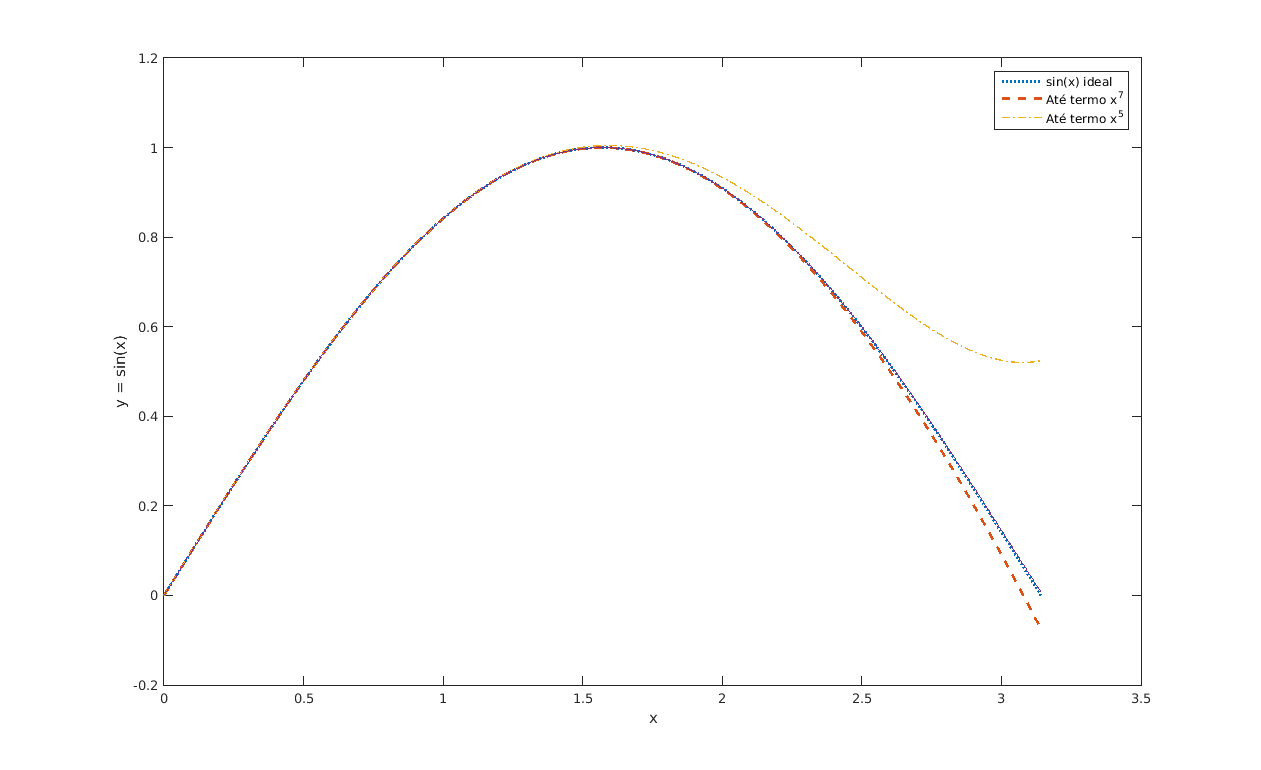
\includegraphics[scale=0.5]{image/sins}
    \caption{Comparação entre seno ideal e séries com número variável de termos}
    \label{img:sins}
\end{figure} 

\FloatBarrier

Por fim, a onda dente de serra é obtida da mesma maneira que a triangular,
exceto que, neste caso, considera-se apenas meio período. O módulo do
coeficiente angular da reta na onda dente de serra é o mesmo daquele na onda
triangular. O código está representado abaixo e a função recebe os mesmos
parâmetros que as funções anteriores.

\begin{lstlisting}[caption= Função de geração de ondas dente de serra.
,language=C, numbers=none] 
void generate_dente_serra_wave(int T, float V) {

	float level, max_level = V/3.3 * 4095;
	int level_int = 0;
	ConversorDA_SetValue(&level_int);

	/* Gera onda ateh usuario pressionar tecla 0 */
	char p  = read_keys();
	while (p != '0') {

		level = 0;
		while ( level < max_level && p != '0') {

			if (p != '0' && p != '#'&& p != '*') p  = read_keys();

			/* max_level * 2 * INTERRUPT_PERIOD / T eh o coeficiente angular */
			level += max_level * 2 * INTERRUPT_PERIOD / T;

			if (level > max_level)	level = max_level;

			level_int = ceil(level);
			ConversorDA_SetValue(&level_int);

			wait_n_interruptions(1); /* Espera 1us */
		}

		/* Suporte as teclas do LCD. */
		if (p != '0' && p != '#'&& p != '*') p  = read_keys();

		/* Aumenta periodo */
		if (p == '*') {
			T += 25000;
			p = 0;
		} /* Diminui periodo */
		else if (p == '#') {
			T -= 25000;
			p = 0;
		}
	}

	level = 0;
	ConversorDA_SetValue(&level);
}
\end{lstlisting}

\section {Implementando um aplicação com o LCD e o DA}

A última etapa envolveu a implementação de uma aplicação que fosse capaz de
selecionar uma das formas segundo tecla apertada pelo usuário (1 para quadrada,
2 para triangular e 3 para senoidal) e ajustar em tempo de execução o período.
As funções apresentadas na seção anterior implementam esta última
funcionalidade: caso \# seja apertado o período da onda diminui em 25ms e, caso
* seja pressionado, o período sofre um incremento de 25ms. O código abaixo
representa a função do nosso programa, que seleciona um dos formatos segundo a
tecla pressionada. As funções \path{send_cmd} e \path{send_string} escrevem e
modificam o estado do LCD, segundo relatório 2.

\begin{lstlisting}[caption= Função \texttt{main}.,language=C, numbers=none] 
for (;;) {
	char wave = read_keys();

	switch (wave) {
	case '1':
		send_cmd(0x01, ceil(1535 / INTERRUPT_PERIOD));
		send_string("Onda Quad.");
		generate_square_wave(250000, 3.3);
		send_cmd(0x01, ceil(1535 / INTERRUPT_PERIOD));
		send_string("Fim onda Quad.");
		break;
	case '2':
		send_cmd(0x01, ceil(1535 / INTERRUPT_PERIOD));
		send_string("Onda Triang.");
		generate_triangular_wave(250000, 3.3);
		send_cmd(0x01, ceil(1535 / INTERRUPT_PERIOD));
		send_string("Fim onda Triang.");
		break;
	case '3':
		send_cmd(0x01, ceil(1535 / INTERRUPT_PERIOD));
		send_string("Onda Senoi.");
		generate_sinoidal_wave(250000, 3.3);
		send_cmd(0x01, ceil(1535 / INTERRUPT_PERIOD));
		send_string("Fim onda Senoi.");
		break;
	}

}
\end{lstlisting}

